\documentclass[conference]{IEEEtran}

\usepackage[noadjust]{cite}
%\usepackage[style=ieee,citestyle=ieee-comp]{biblatex}
\usepackage{amsmath}
\usepackage{graphicx}
\usepackage{tikz-cd}
\usepackage{booktabs}


\title{Explainable AI for Effective Malware Detection and Triage}

\author{\IEEEauthorblockN{Ananta Prasad Gaire, Aleksandar Shurbevski, Shozo Naito}

\IEEEauthorblockA{Kyoto College of Graduate Studies in Informatics (KCGI)\\
Kyoto, Japan\\
Emails: st052439@m2.kcg.edu, a\_shurbevski@kcg.edu, s\_naito@kcg.edu}}

\begin{document}

\maketitle
\begin{abstract}

Security Operations Centers (SOCs) increasingly rely on machine learning to triage large volumes of potentially malicious artifacts, but high-performing models are often difficult to trust because their predictions are opaque.
This paper presents an Explainable AI (XAI) pipeline for static malware detection from Windows Portable Executable (PE) files that combines strong classification performance with analyst-oriented evidence.
The method uses EMBER2024-derived tabular PE features and section-level structural representations rendered as compact ``section images,'' then fuses both modalities for malware/benign classification.
On the held-out full test set (N=960,000), the Tab+ImgEmb LightGBM fusion model achieves ROC-AUC = 0.99795. At the default threshold ($\tau=0.50$), it reaches Accuracy = 0.9795, Precision = 0.9875, Recall = 0.9713, and F1 = 0.9793. At the best-F1 operating point from a 500-threshold sweep ($\tau=0.353$), performance improves to Accuracy = 0.9802, Precision = 0.9829, Recall = 0.9774, and F1 = 0.9801.
To improve decision transparency, the pipeline integrates SHAP for global and per-file explanation of the final LightGBM late-fusion classifier and Grad-CAM for structural evidence from the CNN-based section model, reported in compact tabular form to fit publication constraints.
Results are reported under default and tuned operating thresholds to reflect precision--recall trade-offs relevant to deployment.
Overall, the study shows that high-performing static malware detection can be paired with interpretable evidence artifacts---model scores, ROC-based operating-point analysis, and ranked feature evidence---that support defensible SOC triage.
\end{abstract}

\section{Introduction}
\label{section:introduction}


\subsection{Background and Motivation}

Modern organizations continuously receive, generate, and execute large volumes of digital artifacts through routine workflows such as software distribution, web browsing, and endpoint updates.
In these workflows, Windows Portable Executable (PE) files are especially important from a defensive standpoint because PE is the native executable structure of Windows systems.
PE files remain a dominant malware delivery format and can be distributed through common channels such as downloads, attachments, or bundled installers.
At Security Operations Center (SOCs) scale, the challenge is not only detecting threats but doing so at a speed and volume that manual inspection cannot match.
To handle this scale, SOCs increasingly deploy~\cite{SDRS2025} machine learning (ML) systems to automate triage and prioritize suspicious files for analyst review.
Deep learning models are attractive in this setting because they can learn complex interactions in high-dimensional static features that rule-based filters and signature matching often miss~\cite{DSR2025ai}.
Yet, cybersecurity operations is a high-stakes environment: model outputs often influence decisions such as quarantining endpoints, blocking execution, or escalating incidents.
These actions require accountability.
If a model behaves as a black box and only provides a label (e.g., malware/benign), analysts face a trust gap: either they accept a decision they cannot justify, or they must re-investigate alerts from scratch, which reduces the operational value of automation.
The trust gap grows as threats evolve and adversaries manipulate surface cues.

\subsection{Explainable AI and Why It Matters in Cybersecurity}

Explainable AI (XAI) refers to a family of methods and system designs intended to make the behavior of machine-learning models understandable to humans.
XAI addresses questions such as:
Which inputs contributed most to this prediction?
What evidence increased or decreased the model's confidence? and
What parts of the input were most influential?
In this work, explainability is treated as evidence generation: explanations accompany predictions and support verification, reporting, and analyst reasoning.
This project adopts widely used attribution-based XAI methods because they can be applied directly to trained models without redesigning the model architecture.
For tabular feature inputs and other structured representations, additive feature attribution approaches such as SHapley Additive exPlanations (SHAP)~\cite{LL2017} provide local explanations (why one sample was classified in a certain way) and global summaries (which features are broadly important across many samples).
For tree-based and fused tabular representations, SHAP~\cite{LL2017} provides additive feature attributions that are well aligned with the final classifier used in this work, while Grad-CAM remains appropriate for CNN-based image pathways~\cite{SCDVPB2017}.
For CNN-based components, Grad-CAM produces a saliency heatmap that highlights spatial regions most responsible for a prediction, enabling a visual form of evidence over image-like representations~\cite{SCDVPB2017}.
These methods are well-established and suitable for a pipeline that reports both performance and interpretability.
Explainability matters in cybersecurity for three reasons.
First, it supports trust calibration.
A high confidence score alone is insufficient; analysts must verify that evidence aligns with known malicious patterns.
Second, explainability supports investigation efficiency.
If an alert comes with evidence such as top contributing PE features and highlighted structural regions, analysts can validate or dismiss predictions faster, which improves SOC throughput.
Third, explainability helps reveal failure modes, including shortcut learning, spurious correlations, and inconsistent preprocessing.
In security, these failure modes can be exploited by attackers and can increase false positives.
Therefore, explanations must be validated and interpreted carefully.
This is especially relevant for any saliency signal; prior work cautions that explanation outputs are not automatically faithful and must be evaluated rather than assumed~\cite{JW2019}.

\subsection{Research Aim and Scope}

This research aims to develop and evaluate an explainable, proposal-aligned pipeline for static malware detection from Windows PE artifacts.
The pipeline is designed to produce strong predictive performance and analyst-oriented evidence.
The work focuses on static detection using the EMBER2024 PE feature set~\cite{JMGPR2024} and a section-level structural representation derived from executables.
The scope does not include dynamic malware execution traces, malware family attribution, network intrusion detection, URL crawling, attachment sandboxing, sender reputation systems, or production SOC deployment engineering.

\subsection{Malware Detection Branch: Design and Motivation}

The malware branch investigates explainable static malware detection using the EMBER2024 PE feature representation~\cite{JMGPR2024}.
Structurally, this representation maps each Portable Executable (PE) file into a fixed-dimensional vector of engineered features, summarizing byte-level statistics, header metadata, and import-related information.
The dataset itself directly provides the first modality: a set of tabular descriptors that capture statistical properties of the file.
However, tabular summaries can obscure section-level structural layout information.
To address this, we introduce original descriptors as a second modality by rendering the executable's section layout into a compact image and processing it with a Convolutional Neural Network (CNN).
This allows the system to learn structural patterns not captured by pre-calculated dataset features.
PE files carry both statistical feature evidence (captured by engineered vectors) and structural evidence (captured by section organization), and combining both may strengthen classification while enabling richer explanations.
To evaluate this hypothesis, we train two models: a Tab-only baseline that learns only from the aligned tabular feature vector, and a Tab+ImgEmb model model that merges a feed-forward tabular encoder with a lightweight CNN encoder over section images.
On the held-out test split, the Tab+ImgEmb model model consistently outperformed the Tab-only baseline across both standard and tuned thresholds.

% The comparative results are summarized in Table 1.
% 
% \begin{table}[htbp]
% \centering
% \small
% \setlength{\tabcolsep}{3pt}
% 
% \caption{Performance comparison on EMBER2024 malware detection}
% 
% \begin{tabular}{lccccc}
% 
%     \hline
% \textbf{Model} & \boldmath$\tau$ & \textbf{ACC} & \textbf{F1} & \textbf{ROC-AUC} \\
% \hline
% Tab-only LGBM (EMBERv3) & 0.50 & 0.9794 & 0.9792 & 0.9979 \\
% Tab + ImgEmb LGBM & 0.50 & 0.9795 & 0.9793 & 0.9979 \\
% Tuned Tab + ImgEmb LGBM & 0.35 & 0.9802 & 0.9801 & 0.9979 \\
% \hline
% \end{tabular}
% \label{tab:lgbm_small}

% \end{table}


We emphasize the tuned operating point because threshold selection is operationally important, while still reporting the standard threshold for comparability. Explainability is integrated in a modality-aligned manner.
For the final Tab+ImgEmb LightGBM classifier, we use SHAP to generate explanation evidence over the fused feature vector, including global feature rankings and per-sample feature contributions~\cite{LL2017}.
For the image pathway, we use Grad-CAM~\cite{SCDVPB2017} on the CNN-based section model to generate heatmaps that highlight structurally salient regions in the section-image representation.
During development, we found a reliability issue: missing training-time preprocessing consistency during inference and explainability caused inconsistent probabilities and explanations.
By regenerating and enforcing preprocessing alignment, we restored probability fidelity and kept explanation outputs consistent with the trained pipeline.

\subsection{Contributions}

The main contributions are:
%
\begin{itemize}
\item An explainable multimodal static malware detection pipeline using EMBER2024 PE features, including a Tab-only LightGBM baseline and a Tab+ImgEmb LightGBM late-fusion model evaluated under both standard and tuned thresholds~\cite{JMGPR2024}.
\item A multimodal explanation strategy for malware analysis, combining SHAP for the final LightGBM late-fusion classifier and Grad-CAM for structural localization in the CNN-based section model~\cite{SCDVPB2017,LL2017}.
\item Reliability-focused implementation findings, including strict normalization alignment and feature-schema consistency for stable malware explanations.
\end{itemize}

\section{Related Work}
\label{section:literature-review}

Static malware detection sits at the front line~\cite{KBSSSK2025} of Security Operations Center (SOC) triage because it can be executed quickly, safely, and at scale, often before deeper investigation is feasible~\cite{GPH2024}.
For Windows endpoints, a large share of malicious delivery still arrives as Portable Executable (PE) files~\cite{opentext2025} distributed through downloads~\cite{recordedfuture2025malware}, attachments, and staged droppers.
Defenders must filter high-volume file streams with limited analyst time, and errors are costly.
This highlights the ML ``trust gap.''
Deep models can achieve strong predictive metrics, but SOC decisions still require justification~\cite{NSDSP2025}: why a file was quarantined and what evidence supports that action.
Explainable AI (XAI) addresses this gap by producing interpretable signals (feature attributions and saliency maps) that connect model outputs to concrete input evidence.
In cybersecurity, this evidence supports analyst validation, accelerates investigation, and reduces reliance on opaque automation.
For this reason, this research treats explainability as a first-class system output and evaluates XAI behavior as part of the overall malware detection pipeline~\cite{SCDVPB2017,LL2017}.

\subsection{Static Malware Detection}
\subsubsection{Feature-engineered PE malware detection and the EMBER line of work}

A major practical tradition~\cite{HP20182018} in static malware detection is to extract specific, pre-defined properties from the Portable Executable (PE) file to create a fixed-length input vector.
In the literature, these inputs are variously referred to as ``handcrafted features''~\cite{MT2025,EDS2020}, ``engineered features''~\cite{HP20182018}, or ``tabular descriptors''~\cite{JMGPR2024}.
To maintain consistency and precision, this paper refers to them as engineered features.
These features typically include~\cite{KBSSSK2025} byte-level statistics (e.g., histograms), entropy-related measures that can correlate with packing/obfuscation, metadata derived from headers/sections, and import/export information that reflects program behavior at a coarse structural level.
The key strength of this approach is operational scalability: feature extraction and inference are fast~\cite{EDS2020}, and fixed-dimensional vectors support repeatable benchmarking~\cite{JMGPR2024}, thresholding, and controlled ablation studies~\cite{AQPWPWCR2022}.
The EMBER~\cite{HP20182018} dataset played a foundational role in making large-scale, reproducible PE-feature research possible by providing standardized feature extraction and evaluation conventions.
EMBER2024~\cite{JMGPR2024} extends this tradition by providing a large-scale, pre-computed dataset where each file is represented not as raw bytes, but as a vector of engineered values summarizing specific file characteristics.
These features explicitly include:
Byte-level statistics: Histograms and entropy calculations that capture the distribution of raw byte values.
Header information: Metadata extracted from the COFF and Optional headers (e.g., linker versions, timestamps, and machine types).
Section characteristics: Statistics regarding the size, entropy, and virtual memory layout of the executable's sections.
Import and Export information: Hashed representations of imported libraries, imported functions, and exported symbols, which serve as proxies for the program's capabilities.
By relying on these pre-calculated engineered features, the EMBER2024 representation enables scalable training and systematic evaluation at the feature level~\cite{JMGPR2024,HP20182018}.
Benchmark baselines and published results.
To support reproducible comparison, the EMBER2024 authors also provide official benchmark models and runnable training/evaluation scripts in the public repository (see the examples/ directory)~\cite{JMGPR2024,ember2024github}.
These baselines are primarily LightGBM classifiers trained on EMBER feature version 3 vectors, intended to serve as reference performance levels for future work.
For malicious/benign detection, the benchmark LightGBM classifier achieves ROC AUC = 0.9949 and reaches a true positive rate of 94.48\% at a 1\% false positive rate on the EMBER2024 test set~\cite{JMGPR2024}.
For malware family classification, the benchmark LightGBM model reports accuracy = 67.97\%, with weighted-F1 = 0.6664 and macro-F1 = 0.4371, reflecting the long-tail difficulty across many smaller families~\cite{JMGPR2024}.
These published baseline results provide a consistent reference point that later experimental results (including ours) should be compared against.

\subsubsection{Representation learning from raw bytes and the ``end-to-end'' alternative}

In parallel to engineered-feature pipelines, a competing research direction~\cite{RBSBCN2017,KBSSSK2025} argues that end-to-end models operating directly on raw bytes can discover discriminative patterns without relying on explicit feature design.
MalConv~\cite{RBSBCN2017} is a widely cited example of this idea~\cite{MT2025,EDS2020}, demonstrating that convolutional architectures can ingest long byte sequences to classify executables.
This family of approaches has expanded the field's understanding~\cite{RCEJH2025,KBSSSK2025} of representation learning for malware, but it also highlights practical constraints that are important for SOC-facing systems: very long sequences increase compute and memory costs~\cite{EDS2020}, truncation or padding choices can affect what the model learns~\cite{RBSBCN2017,AQPWPWCR2022}, and mapping byte-level signals to analyst-friendly evidence can be challenging compared to structured PE features~\cite{NSDSP2025,AQPWPWCR2022}.
These trade-offs matter to our project design.
We stay within a controlled, fixed-dimensional representation (tabular PE vectors, plus a compact ``section image'' representation) to keep the pipeline scalable and explanation outputs interpretable.
In other words, rather than choosing between ``feature engineering'' and ``end-to-end bytes,'' our work aligns with literature~\cite{JMGPR2024,RBSBCN2017} that treats representation choice as an operational design decision: maintain tractable inputs that can support stable training, controlled evaluation, and explanation artifacts that analysts can act on.

\subsubsection{Malware-as-image and structural visual encodings}

Another influential branch~\cite{NKJMB2011,KBSSSK2025} of malware research transforms executables into image-like representations to enable CNN-based modeling.
Early work~\cite{NKJMB2011} showed that visualizing binaries as images can support classification by capturing texture-like patterns that emerge from byte structure.
More recent work~\cite{ZLSC2024} continues to explore image conversion techniquesnsometimes combined with additional features---showing that visual encodings can complement other representations when designed carefully.
The literature further establishes that image-based approaches offer distinct advantages for interpretability and fusion.
Research indicates that unlike purely tabular data, visual representations enable spatial explanation methods (e.g., Grad-CAM) that can highlight exactly which regions of a file structure influence the model's decision~\cite{SCDVPB2017,ZLSC2024}.
Furthermore, studies in multimodal learning suggest that combining these structural visual signals with engineered feature vectors creates a more robust detection system, as the two modalities capture complementary patterns statistical evidence from features and spatial evidence from structure ~\cite{NKJMB2011,ZLSC2024}.

\subsubsection{Multimodal and fusion modeling for static malware detection}

The literature increasingly suggests~\cite{ZLSC2024,KBSSSK2025} that no single static view fully captures malware behavior, especially under packing, obfuscation, and family diversity.
As a result, fusion architectures that combine complementary signals have become more common.
For example, research that jointly analyzes PE structure with entropy-related signals reflects the broader idea that combining structural and distributional properties can improve malware classification robustness~\cite{SZS25}.
More generally, fusion is attractive because it provides redundancy: when one modality is less informative for a sample (e.g., a heavily packed file), another modality may still retain useful evidence.
This trajectory in malware research supports the hypothesis that fusing structured PE vectors with compact structural visual representations can improve detection performance without abandoning interpretability~\cite{SZS25,SCDVPB2017}.
By comparing tabular-only baselines against fusion architectures, recent studies aim to quantify exactly how much robustness is gained by integrating these complementary static views.

\subsubsection{Explainability for malware: feature attribution for the final classifier and localization for the CNN pathway}

As explainable AI becomes increasingly important in malware detection~\cite{KBSSSK2025,NSDSP2025}, explanation methods must be matched to the actual model architecture used at inference time.
In the implemented pipeline, the final malware decision is produced by a LightGBM late-fusion classifier rather than an end-to-end neural network.
Accordingly, additive feature attribution methods such as SHAP are better aligned with the final classifier because they quantify how each fused feature contributes to the model score~\cite{LL2017}.
For malware detection, this produces ranked feature evidence that can be summarized into analyst-readable tables at both global and per-sample levels.

For CNN-based components, Grad-CAM produces class-discriminative heatmaps that highlight which spatial regions in an image-like input most strongly influenced the network response~\cite{SCDVPB2017}.
For section-image encodings, this provides a useful ``where the model looked'' signal over the structural representation.
However, in the implemented pipeline, Grad-CAM is applied to the CNN-based section model used to produce image-side evidence, while SHAP is used to explain the final LightGBM classifier.
This distinction is important because it separates explanation of the final decision from supporting structural evidence in the image pathway.

A critical point in XAI literature~\cite{DJRLXSWB2020,NSDSP2025} especially relevant to security is that explanation outputs must be reliable, not merely visually appealing.
Sanity-check research shows that some saliency or explanation methods can fail in subtle ways (e.g., remaining similar even when model parameters or labels are randomized), motivating validation procedures rather than assuming explanation faithfulness by default~\cite{JJMIMB2018}.
This supports the methodological choice to treat explanation generation and validation as part of system design rather than as a post-hoc screenshot~\cite{SCDVPB2017,LL2017,JJMIMB2018}.

\subsection{Summary and Positioning}

The malware literature shows a consistent trajectory: high-performing models increasingly rely on deep learning and richer representations, but operational adoption in cybersecurity still requires transparent evidence and explanation reliability.
EMBER-style PE feature benchmarks and multimodal fusion trends motivate our Tab-only baseline and Tab+ImgEmb late-fusion design, while SHAP and Grad-CAM provide explanation modalities aligned to the implemented pipeline~\cite{JMGPR2024,SZS25,SCDVPB2017,LL2017,HP20182018,NKJMB2011}.
This section motivates controlled and scalable representations, multimodal fusion, and measurable explanation outputs aligned with the implemented pipeline~\cite{JMGPR2024,SZS25,SCDVPB2017,LL2017,JJMIMB2018}.


\section{Methodology}
\label{section:methodology}

This paper proposes and evaluates an Explainable AI (XAI) framework for static malware detection from Portable Executable (PE) artifacts.
The methodology reflects SOC requirements: high-volume detection under time constraints, with evidence for analyst validation and reporting.
The project treats explainability as a core output, not a post-hoc visualization, because security decisions require justification and traceability.
The methodology emphasizes scalability and multimodal evidence, using large-scale PE feature vectors and section-derived structural representations to study whether complementary static views improve robustness.
Evaluation is conducted under a consistent protocol and includes probability threshold analysis to reflect deployment-style trade-offs in security settings.

\subsection{Malware Detection}
\subsubsection{Data Source and Dataset Representation}

The malware branch is implemented as a static detection problem using an EMBER2024-derived PE feature representation~\cite{JMGPR2024}, grounded in the broader EMBER benchmark tradition of large-scale, reproducible PE malware research~\cite{HP20182018}.
Each executable is represented as a fixed-dimensional feature vector extracted from intrinsic properties of the PE artifact, and each sample is assigned a binary label indicating benign or malicious class membership.
This representation is suitable for security triage because it supports efficient batch inference and allows structured explanation outputs at the feature level.
To support large-scale processing, the dataset is organized in a sharded format where each shard stores a feature matrix and corresponding labels.
Formally, each shard contains a feature matrix and a label vector, enabling streaming-style loading and memory-safe inference.
This structure is important because the dataset scale requires repeated passes for training, validation, testing, and explainability generation without relying on full in-memory loading.
A key implementation detail in this project is strict control of the effective feature dimension used by trained models and explainability routines.
In the final code-backed pipeline, the tabular branch uses the EMBERv3 feature vector, and the LightGBM experiments are reported on the full tabular representation used by the released scripts.
This alignment step is necessary because neural network layers are parameterized for a specific input dimensionality, and even a single-feature mismatch prevents strict model reuse and can lead to inconsistent explanations.

\subsubsection{Preprocessing and Normalization}

Feature scaling is treated as a first-order methodological requirement because deep models trained on heterogeneous feature groups can become unstable or misleading if preprocessing differs between training, inference, and XAI computation.
In this project, feature normalization statistics are computed on the training split and reused consistently in all later steps.
Let and denote the per-feature mean and standard deviation estimated from training data.
For each enforced input vector, the normalized vector is computed as:
where is a small constant to prevent division-by-zero.
This project explicitly enforces preprocessing consistency because explanation reliability depends on the model operating in the same numerical feature space that it was trained on.
Inconsistent normalization can change predicted probabilities and distort gradient-based explanations, which undermines the central objective of producing analyst-usable evidence.

\subsubsection{Model Architectures}

To evaluate the benefit of multimodal evidence while retaining interpretability, the project implements two complementary architectures: a tabular baseline and a multimodal fusion model.
Both operate on the same normalized tabular features, and the fusion model additionally incorporates a compact structural representation processed by a CNN.
Tabular-only neural classifier (Tab-only)
The baseline model is a deep tabular classifier that maps normalized PE feature vectors to class logits.
Let denote the network with parameters, and let be the output logits for the benign and malware classes.
The malware probability is computed using the softmax mapping:
This baseline quantifies how much discriminative power is available from tabular PE features alone under the project's normalization and evaluation protocol.
Multimodal late-fusion classifier (Tab+ImgEmb LightGBM)
The final fusion model combines two sources of evidence: the normalized EMBER tabular feature vector and an exported image embedding derived from a CNN-based section model operating on section-structure representations.
For each sample, the tabular feature vector is concatenated with the image embedding to form a late-fusion feature vector, which is then passed to a LightGBM classifier to produce the final malware probability.
This design preserves the complementary strengths of the two modalities: tabular PE features capture global structural and statistical signals, while the CNN-based section model captures structural patterns that are summarized into the image embedding.
Importantly for this research, the explainability pipeline is aligned to this implementation: SHAP explains the final LightGBM decision, while Grad-CAM provides complementary structural evidence from the CNN-based section model~\cite{LL2017,SCDVPB2017}.

\subsubsection{Evaluation Protocol and Operational Thresholding}

Evaluation is performed on a held-out test split that contains 960,000 samples in the finalized experiment configuration.
For each test sample, the model outputs a malware probability.
A decision threshold converts probability into a binary prediction:
The project reports performance under the conventional operating point and additionally performs a threshold sweep to select an operating threshold optimized for the malicious class F1 score.
This selection is formalized as:
The purpose of this step is not to ``inflate'' metrics but to reflect how SOC deployments often require tuned decision boundaries depending on tolerance for false positives versus missed detections.
The methodology therefore preserves transparency by reporting both the default threshold and the best-F1 threshold.

\subsubsection{Explainability Methods}

We use two explanation methods aligned with the implemented malware pipeline: SHAP for the final LightGBM late-fusion classifier and Grad-CAM for the CNN-based section model~\cite{LL2017,SCDVPB2017}.

For the final classifier, the input to LightGBM is a late-fusion vector formed by concatenating the EMBER tabular feature vector with the exported image embedding from the section model.
SHAP is applied directly to this trained tree-based model to measure how each fused feature dimension contributes to the malware score.
Global explanations are produced by computing mean absolute SHAP values over an explained sample subset, yielding a ranked summary of the most influential fused features.
The implementation supports SHAP-based explanation of the final classifier and saves global summary artifacts, while the same SHAP framework can also be used for per-sample analyst review.

Grad-CAM is not applied to the final LightGBM classifier itself.
Instead, it is applied to the CNN image pathway within the trained section model used to generate image-side evidence.
This produces a class-discriminative heatmap over the section-image representation, highlighting which structural regions were emphasized by the CNN pathway.
In this way, SHAP explains the final late-fusion decision, while Grad-CAM provides complementary structural evidence from the image side of the system.


\section{Implementation and Results}
\label{section:implementation-and-results}


We implemented two malware detection models operating on engineered static PE feature representations.
The baseline model is a Tab-only LightGBM classifier that consumes a fixed-length numeric feature vector and outputs a malware probability.
The main model is a Tab+ImgEmb LightGBM late-fusion classifier that augments the same tabular evidence with an image embedding exported from a CNN-based section model trained on a compact section-structure representation.
The design goal is practical: keep inference scalable for millions of files while producing analyst-facing evidence rather than a single opaque score.

\subsubsection{Decision Rule, Threshold Sweep, and Reported Metrics}

For each test sample $i$, the model outputs a malware probability $p_i = p(y=1 \mid x_i)$.
Given a decision threshold $\tau$, the predicted label is $\widehat{y}_i(\tau)=1$ if $p_i \geq \tau$ and 0 otherwise.
From the resulting confusion matrix counts, we compute Accuracy, Precision (malicious), Recall (malicious), and F1 (malicious).
Because operational malware detection often requires balancing false negatives (missed malware) against false positives (benign files escalated), we report results at the conventional $\tau=0.50$ and also report the best-F1 operating point identified by sweeping $\tau$ over multiple values.

\subsubsection{Final Test Performance}

Table~\ref{tab:model_comparison} summarizes the final test performance for the Tab-only baseline and the Tab+ImgEmb fusion model on the full EMBER2024 test set.
The fusion model is reported as the primary outcome, while the tabular-only model provides a reference point for quantifying the contribution of the image-embedding branch.

To contextualize these results, we compare them with the official EMBER2024 benchmark reported by Joyce et al. and distributed with example scripts [1, 37].
The published malicious/benign baseline is reported using threshold-independent operating metrics (ROC AUC = 0.9949 and TPR = 94.48\% at 1\% FPR) [1].
Although this paper reports thresholded metrics at $\tau = 0.50$ and at the best-F1 operating point, the comparison remains useful because it shows that the proposed system preserves strong separability while also providing analyst-oriented explanations.

\begin{table}[htbp]
\centering
\caption{Final malware detection results on the full EMBER2024 test set (N=960,000).}
\label{tab:model_comparison}
\small
\setlength{\tabcolsep}{4pt}
\begin{tabular}{lcccccc}
\hline
\textbf{Model} & \boldmath$\tau$ & \textbf{AUC} & \textbf{ACC} & \textbf{Prec.} & \textbf{Recall} & \textbf{F1} \\
\hline
Tab-only LGBM (EMBERv3 2568) & 0.50  & 0.997938 & 0.979406 & 0.9877 & 0.9709 & 0.9792 \\
Tab+ImgEmb LGBM              & 0.50  & 0.997949 & 0.979481 & 0.9875 & 0.9713 & 0.9793 \\
Tab+ImgEmb LGBM (best-F1)    & 0.353 & 0.997949 & 0.980175 & 0.9829 & 0.9774 & 0.9801 \\
\hline
\end{tabular}
\end{table}


Figure~\ref{fig:roc_curve} shows the ROC curve of the final Tab+ImgEmb model on the full test set.
The model achieves ROC-AUC = 0.99795, indicating strong class separability across operating thresholds.
This threshold-independent view complements the fixed-threshold metrics in Table~\ref{tab:model_comparison}.

\begin{figure}[htbp]
    \centering
    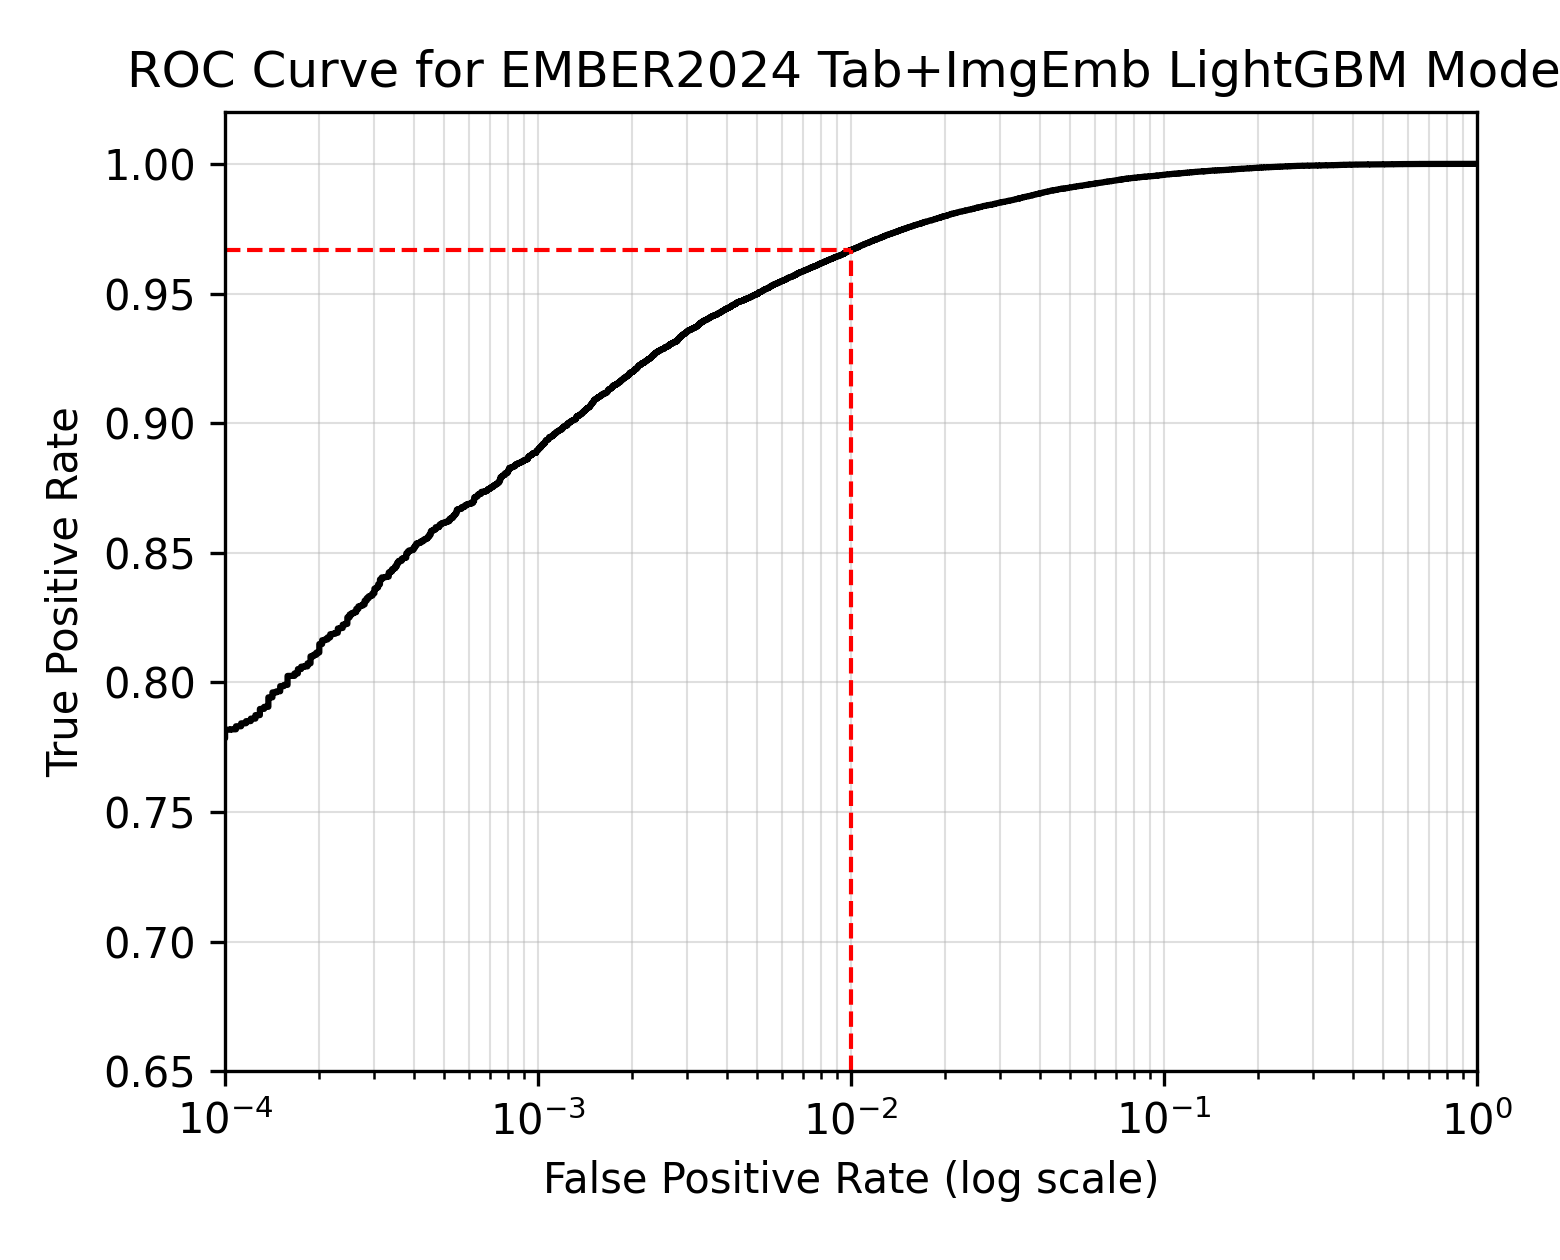
\includegraphics[width=0.4\textwidth]{curves/ROC_tab_plus_imgemb_full_test.png}
    \caption{ROC curve of the final Tab+ImgEmb LightGBM model on the EMBER2024 full test set (AUC = 0.99795).}
    \label{fig:roc_curve}
\end{figure}

The main takeaway is that the fusion model improves recall and F1 while maintaining strong precision, which is important for malware triage where missed malware is typically more costly than additional analyst review.



%Figure 4.1 provides a compact visualization of the same comparison.
The main takeaway is that fusion improves recall and F1, meaning it catches more malicious samples while maintaining strong precision.
%Figure 4.1.
Malware performance comparison (Accuracy, F1, Recall) for Tab-only and Fusion at two operating points.

\subsubsection{Operational Interpretation}

Table~\ref{tab:operational_counts} translates threshold choices into tangible operational costs.
In malware triage, False Negatives (FN) correspond to malware that evades blocking and reaches endpoints, while False Positives (FP) correspond to benign files that are incorrectly quarantined or escalated.
At the default threshold, the model keeps the false-positive rate low while still achieving strong recall.
At the best-F1 operating point, false negatives are reduced further, at the cost of a moderate increase in false positives.

\begin{table}[htbp]
\centering
\caption{Operational counts for the final Tab+ImgEmb model on the full EMBER2024 test set.}
\label{tab:operational_counts}
\small
\setlength{\tabcolsep}{4pt}
\begin{tabular}{lcccccc}
\hline
\textbf{Setting} & \boldmath$\tau$ & \textbf{TN} & \textbf{FP} & \textbf{FN} & \textbf{TP} & \textbf{FPR} \\
\hline
Default threshold & 0.50  & 474094 & 5906 & 13792 & 466208 & 0.0123 \\
F1 threshold & 0.353 & 471816 & 8184 & 10848 & 469152 & 0.0171 \\
\hline
\end{tabular}
\end{table}

Table~\ref{tab:operational_counts} shows the practical trade-off clearly.
At $\tau=0.50$, the model misses 13,792 malware samples while keeping false positives to 5,906 benign files.
At $\tau=0.353$, false negatives drop to 10,848, improving recall, while false positives rise to 8,184.
This trade-off is useful for deployment because threshold selection can be matched to whether missed malware or analyst workload is considered more costly.

\subsubsection{Explainability Report for Malware}

To make malware decisions reviewable, we summarize explanations in a compact tabular format aligned with the implemented late-fusion architecture.
For the final Tab+ImgEmb LightGBM classifier, SHAP provides signed feature attributions over the fused input vector, where positive values increase the malware score and negative values decrease it.
To save space, explanation evidence is reported as ranked tables rather than multiple heatmap figures.
This allows the paper to preserve the decision-support value of the explanations while meeting the page limit.

Global SHAP summary (model-wide feature importance).
Global SHAP shows which fused features consistently influence predictions across many samples.
Table 4.2 lists the top-ranked features by mean absolute SHAP magnitude.
Even when feature identifiers are generic, this ranking remains valuable for reproducibility and for later mapping to broader groups such as tabular PE statistics and image-embedding dimensions.

\iffalse
\begin{table}[htbp]
\centering
\caption{Top-ranked global mean absolute SHAP features for the Tab+ImgEmb LightGBM model.}
\label{tab:feature_rank}

\begin{tabularx}{\columnwidth}{clX} % 'X' makes the feature column flexible
\toprule
\textbf{Rank} & \textbf{Feature} & \textbf{Mean $|SHAP|$} \\
\midrule
1  & byte\_feature\_217    & 0.7432 \\
2  & byte\_feature\_105    & 0.7342 \\
3  & section\_feature\_512 & 0.6146 \\
4  & section\_feature\_435 & 0.4992 \\
5  & byte\_feature\_103    & 0.4979 \\
6  & section\_feature\_256 & 0.3981 \\
7  & byte\_feature\_145    & 0.3909 \\
8  & byte\_feature\_129    & 0.3849 \\
9  & byte\_feature\_124    & 0.3686 \\
10 & section\_feature\_486 & 0.3637 \\
\bottomrule
\end{tabularx}

\end{table}

%Table 4.2.
Top-ranked global mean absolute SHAP features for the Tab+ImgEmb LightGBM model.
\fi

Local explanation summary: four representative case studies.

Local explanations are critical for incident response because analysts validate individual alerts.
We therefore summarize four representative test cases using compact explanation tables.
These examples were selected to cover different decision regimes: low-confidence malware, high-confidence benign, high-confidence malware, and a borderline benign case near common operating thresholds.

Table 4.3 summarizes the local explanation evidence for four representative malware samples.
POS increases malware probability, while NEG decreases it.
A useful detail in interpreting Table 4.3 is that SHAP explanations are signed, so they naturally show both supporting and suppressing evidence.
In other words, the model may detect some benign-leaning signals even in a malware sample, but the final probability reflects the net effect of all evidence.
This push-pull behavior is particularly informative for borderline cases because it reveals why the model hesitated.

\subsubsection{What the Malware Results Mean}

The malware results support three conclusions.
First, the Tab+ImgEmb LightGBM late-fusion model consistently outperforms the tabular-only baseline, indicating that the image-embedding branch contributes complementary information rather than redundant noise.
Second, the improvement is especially meaningful in recall: at $\tau=0.50$, the fusion model misses fewer malicious samples, which is important because false negatives are often the more costly error in security operations.
Third, compact explanation tables help justify decisions in uncertain cases by showing how malware-leaning and benign-leaning evidence compete near the operating threshold, which is exactly where analyst review is most valuable.

\section{Conclusion and Future Work}
\label{section:conclusion-and-futurework}

This paper presents an explainable static malware detection pipeline that combines tabular EMBER2024 features with image embeddings derived from section-structure representations.
Across experiments, the Tab+ImgEmb fusion model outperformed the tabular-only baseline, with the most important operational gain being lower false negatives.
On the full EMBER2024 test set (N=960,000), the Tab+ImgEmb model achieved ROC-AUC = 0.99795.
At the default threshold ($\tau=0.50$), the model reached Accuracy = 0.9795, Precision = 0.9875, Recall = 0.9713, and F1 = 0.9793.
At the best-F1 operating point from the 500-threshold sweep ($\tau=0.353$), performance improved to Accuracy = 0.9802, Precision = 0.9829, Recall = 0.9774, and F1 = 0.9801.
These results support treating threshold selection as an explicit deployment policy choice rather than a fixed default.

The explainability layer improved interpretability of model behavior.
SHAP provided directional feature attributions for the final LightGBM late-fusion classifier, and Grad-CAM provided structural localization for the CNN-based section model used to generate image-side evidence.
To keep the paper concise, explanation results are summarized as compact tables rather than multiple heatmap figures.
A key implementation finding was that strict preprocessing and feature-schema alignment are required for stable probabilities and reproducible explanations.

The results should be interpreted within clear boundaries.
The evaluation used a prepared split and static labels, so external validity under evolving malware distributions remains an open question.
Feature-schema consistency across dataset preparation, inference, and explanation generation highlighted the importance of strict version and preprocessing control in practical malware pipelines.
In addition, attribution outputs should be treated as supporting evidence, not causal proof.

Future work should prioritize deployment-oriented extensions: (i) richer semantic mapping of fused features and broader evaluation (calibration, precision--recall analysis, and time-split/family-level tests), (ii) standardized analyst evidence cards combining score, decision, top SHAP attributions, and Grad-CAM, and (iii) monitoring/governance for performance drift, explanation drift, dataset versions, feature schemas, and threshold settings.

% \section*{Acknowledgment}
% The authors thank the Kyoto College of Graduate Studies for Informatics for providing access to computing facilities in support of this research.

\bibliographystyle{IEEEtran}

\bibliography{references}

\end{document}
